\section{Motivation}
\label{sec:motivation}

In this section, we motivate our research by outlining a few concrete real-world
applications

\subsection{Motivating Applications}
\label{sec:motiv-appl}

We consider three distinct area, yet architecturally similar applications. These
applications represent the streaming applications that span the wide area and
the traditional ways have been aggregating them and processing offline.

\subsubsection{Smart City}
\label{sec:smart-city}

\todo{ask for Shenzhen's data}

\subsubsection{Continuous Visual Event Recognition}
\label{sec:cont-visu-event}

We use VIRAT Video Dataset~\cite{oh2011large} and count the number of people in
each frame. Such application can be useful in retail stores or large shopping
malls.

\subsubsection{Log Monitoring}
\label{sec:log-monitoring}

\todo{Conviva Log}.

\subsection{Making the Case for Adaptive Execution}
\label{sec:making-case-adapt}

Describe how the wide-area network resources fluctuate, Even well-provisioned
bandwidth between data centers.

\begin{figure}
  \centering
  \begin{subfigure}{.48\columnwidth}
    \centering
    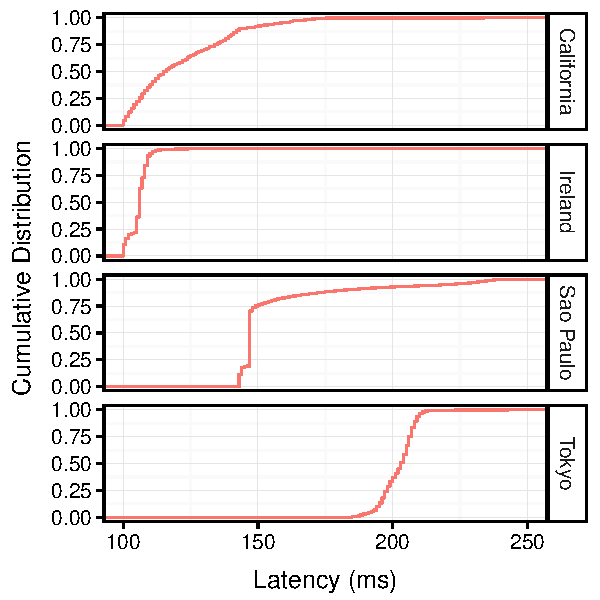
\includegraphics[width=.95\linewidth]{figures/latency-cdf.pdf}
    \caption{CDF}
    \label{fig:bar}
  \end{subfigure}
  \begin{subfigure}{.48\columnwidth}
    \centering
    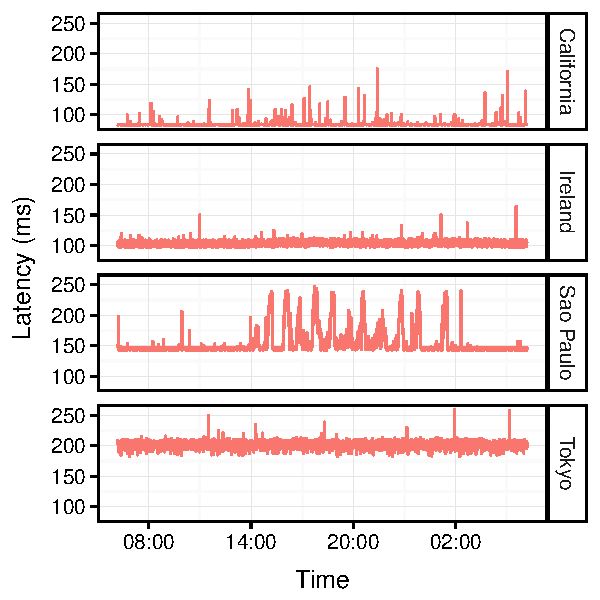
\includegraphics[width=.95\linewidth]{figures/latency-ts.pdf}
    \caption{Timeseries plot}
    \label{fig:ts}
  \end{subfigure}
  \caption{Measured from Ireland, data from PBallis's measurement}
  \label{fig:bw}
\end{figure}

\begin{figure}
  \centering
  \begin{subfigure}{.48\columnwidth}
    \centering
    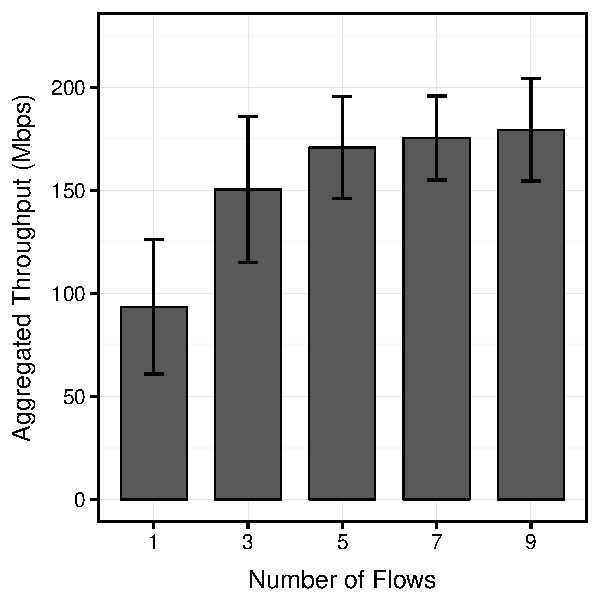
\includegraphics[width=.95\linewidth]{figures/bw-bar.pdf}
    \caption{Bar plot}
    \label{fig:bar}
  \end{subfigure}
  \begin{subfigure}{.48\columnwidth}
    \centering
    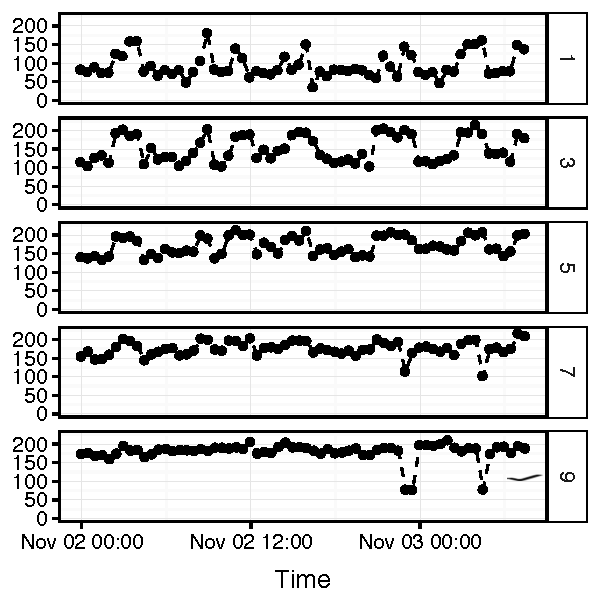
\includegraphics[width=.95\linewidth]{figures/bw-ts.pdf}
    \caption{Timeseries plot}
    \label{fig:ts}
  \end{subfigure}
  \caption{Bandwidth fluctuations from Europe EC2 (Ireland) to US-East
    (Virginia)}
  \label{fig:bw}
\end{figure}

Although the latency is mostly stable.

Application can transmit a large chunk of data if needed. But when the network
condition deteriorate, doing so will create back-logged data. Not all sensor
data and log data are inheritantly important, many application can tolerate data
loss. So we could degrade the data quality but remains responsive.

%% Maybe also last hop wireless?

%%% Local Variables:
%%% mode: latex
%%% TeX-master: "sigcomm2017"
%%% End:
